\documentclass{article}
\usepackage[paperwidth=120cm,paperheight=72cm,margin=0cm]{geometry}
\usepackage[T1]{fontenc}
\usepackage{lmodern,amsmath,amssymb,graphicx,xcolor,tikz,booktabs}
\usepackage[colorlinks=true,urlcolor=navy]{hyperref}
\renewcommand{\familydefault}{\sfdefault}
\pagestyle{empty}
\definecolor{navy}{HTML}{003E72}
\definecolor{captionblue}{HTML}{547A9B}
\definecolor{rulegrey}{HTML}{A9B3BD}
\setlength{\parindent}{0pt}
\setlength{\parskip}{0.28cm}
\newcommand{\heading}[1]{\par\vspace{0.55cm}{\color{navy}\bfseries\fontsize{30}{35}\selectfont #1\par}\vspace{0.12cm}{\color{rulegrey}\hrule height 0.7pt}\vspace{0.32cm}}
\newcommand{\step}[1]{\par\vspace{0.25cm}\textbf{\color{navy}#1}\par}
\newcommand{\figcap}[2]{{\color{captionblue}\fontsize{20}{25}\selectfont\textbf{Figure #1.} #2\par}\vspace{0.3cm}}
\newcommand{\fig}[2]{\begin{center}\includegraphics[width=#2\linewidth]{figures/#1.pdf}\end{center}}
\newsavebox{\leftcolumn}\newsavebox{\middlecolumn}\newsavebox{\rightcolumn}
\begin{document}
\fontsize{23}{29}\selectfont
\setlength{\abovedisplayskip}{0.24cm}\setlength{\belowdisplayskip}{0.24cm}
\setlength{\abovedisplayshortskip}{0.18cm}\setlength{\belowdisplayshortskip}{0.18cm}

\begin{lrbox}{\leftcolumn}\begin{minipage}[t]{36cm}\raggedright

  \heading{Introduction to Tilings}

    Let \(\mathcal{T}=\{T_\alpha\}_{\alpha\in A}\) be a collection of subsets of the Euclidean plane \(\mathbb{R}^2\).
We say that \(\mathcal{T}\) is \textbf{a \emph{tiling} (or \emph{tessellation})} if the following three conditions hold:
\begin{enumerate}
  \item \textbf{Covering (no gaps):}
        \[
          \bigcup_{\alpha\in A} T_\alpha \;=\; \mathbb{R}^2.
        \]
  \item \textbf{Non-overlap:} for every \(\alpha\neq\beta\),
        \[
          \operatorname{int}(T_\alpha)\;\cap\;\operatorname{int}(T_\beta)=\varnothing,
        \]
        where \(\operatorname{int}(\,\cdot\,)\) denotes the interior.
  \item \textbf{Topological disks:} each tile \(T_\alpha\) is \emph{homeomorphic}
        to the closed unit disk \[
        D^2=\{(x,y)\in\mathbb{R}^2:\,x^2+y^2\le 1\}
        \]
        \end{enumerate}

  \heading{Fundamentals of Penrose Tiling}
    Penrose tilings are \textbf{non-periodic tilings} discovered by mathematician and physicist Roger Penrose in the 1970s. Unlike regular periodic tilings (like squares or hexagons), Penrose tilings:

\begin{itemize}
    \item \textbf{No Translational Symmetry} -- no nonzero translation preserves the entire tiling; finite patches do recur.
    
    \item \textbf{Can be constructed using different rules} -- for example, matching rules and projection methods (e.g., de Bruijn's pentagrid approach)

    \end{itemize}
\begin{center}
\begin{minipage}{0.44\linewidth}\centering
\figcap{1}{Basic Penrose Rhombic Tiles}
\resizebox{\linewidth}{!}{\begin{tabular}{lcc}\toprule
\textbf{Tile Type}&\textbf{Angles}&\textbf{Edge Length}\\\midrule
Thin Rhombus&$36^\circ,144^\circ$&Equal\\
Thick Rhombus&$72^\circ,108^\circ$&Equal\\\bottomrule
\end{tabular}}
\end{minipage}\hfill
\begin{minipage}{0.53\linewidth}\centering
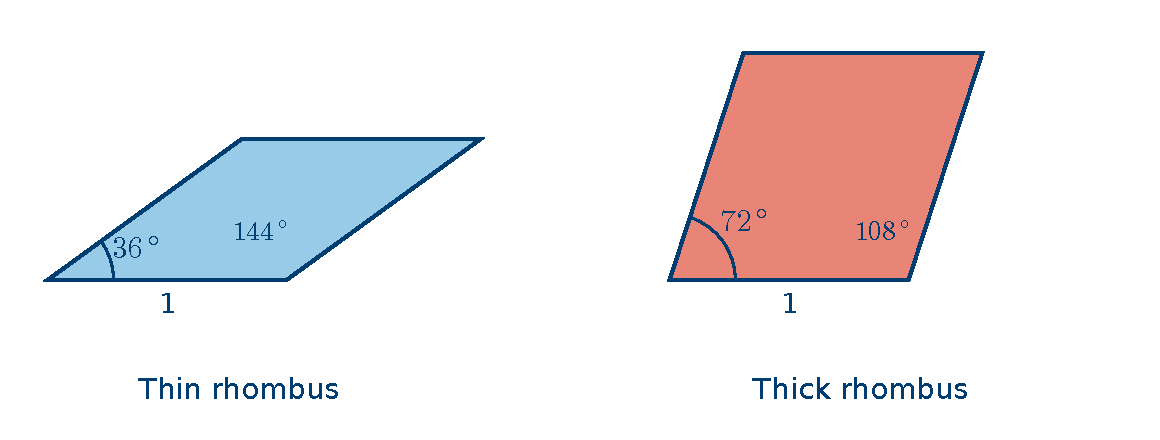
\includegraphics[width=\linewidth]{figures/figure2-prototiles.pdf}
\figcap{2}{Basic Penrose Rhombic Tiles}
\end{minipage}\end{center}

  \heading{Pentagrid Patterns}
Each rhomb has \textbf{two pairs of parallel edges}, you can chain rhombs edge-to-edge along any one pair and \textbf{create a long ``ribbon''}.

There are only \textbf{five distinct edge directions} in the Penrose rhomb set, so \textbf{ribbons within the same family do not intersect with each other} .

    \fig{figure3-ribbon}{0.98}
\figcap{3}{Pentagrid and Tiling. A highlighted grid line corresponds to a ribbon of rhombi.}

\textbf{de Bruijn} found that the ribbons can be reconstructed into sets of parallel lines, which is called \textbf{pentagrid}. While the \textbf{intersections of 2 lines} in the pentagrid pattern can be represented \textbf{a particular rhomb}.

\end{minipage}\end{lrbox}
\begin{lrbox}{\middlecolumn}\begin{minipage}[t]{36cm}\raggedright

  \heading{Constructing Penrose Tilings with Pentagrid}
\textbf{1.  Five grids} \smallskip  
For $j=0,\dots,4$ , set the unit direction vectors
\[
v_{j}=\bigl(\cos 2\pi j/5,\;\sin 2\pi j/5\bigr),\qquad
\gamma_{0}+\dots+\gamma_{4}=0 .
\]
The $j$-th line family is  
\[
\mathcal L_{j}=\bigl\{\,x\in\mathbb R^{2}\ \big|\ x\!\cdot\!v_{j}+\gamma_{j}\in\mathbb Z\bigr\}.
\]

    \fig{figure4-directions-grid}{0.95}
\figcap{4}{de Bruijn's Pentagrid and its Corresponding Vectors. Adjacent vectors are separated by $2\pi/5$.}
 
The pentagrid is called \textbf{regular} if no point of $\mathbb R^2$ belongs to \textbf{more than two of the five grids}, and otherwise singular.

\medskip
\textbf{2.  Integer coordinates of a cell} \smallskip  
For any $x\in\mathbb R^{2}$, define the integer-valued functions
\[
K_{j}(x)=\bigl\lceil\,x\!\cdot\!v_{j}+\gamma_{j}\bigr\rceil,
\qquad
K(x)=(K_{0},\dots,K_{4})\in\mathbb Z^{5}.
\]
where:
 $\gamma_j$ are the grid shift parameters

\medskip
$K(x) = (K_{0}(x), . . . ,K_{4}(x))$ is a five-tuple, which are representing the \textbf{``pentagrid coordinates of a vertex in the tiling''}.\\
\smallskip
The map $x\mapsto K(x)$ is \textbf{constant} on each open cell and they change only when \textbf{crossing a grid line}.

\fig{figure5-cell-coordinates}{0.95}
\figcap{5}{Coordinates in Pentagrid. Four neighbouring cell labels project to the vertices of a rhombus.}

\medskip
\textbf{3.  Linear projection to the plane}\smallskip  
\[
f\bigl(k_{0},\dots,k_{4}\bigr)=\sum_{j=0}^{4}k_{j}\,v_{j}
\]

The $K(x)$ act as ``coordinates'' in a 5D space, and $f(K(x))$ projects them to 2D. The resulting point $f(K(x))$ is a vertex in the Penrose tiling.

\medskip

\end{minipage}\end{lrbox}
\begin{lrbox}{\rightcolumn}\begin{minipage}[t]{36cm}\raggedright

    \heading{(Continue) Constructing Penrose Tilings with Pentagrid}

\textbf{4.  Each two-line crossing gives one rhomb.} \smallskip  
 Choose $0\le r<s\le4$ and integers $k_{r},k_{s}$.  Solving
\[
v_{r}\!\cdot x+\gamma_{r}=k_{r},
\qquad
v_{s}\!\cdot x+\gamma_{s}=k_{s}
\]
gives an \textbf{intersection} $x_{0}$.  

For example, given the \textbf{five-tuple} $K(x_{0})=(K_{0},\dots,K_{4})$ and the pair
$(r,s)=(0,1)$, the \textbf{four vertices} correspond to  
\[
K(x_{0})+(\varepsilon_{1},\;\varepsilon_{2},\;0,\;0,\;0),
\qquad
\varepsilon_{1},\varepsilon_{2}\in\{0,1\}.
\]

Thus, we apply \textbf{the linear map}
\(
f(k)=\sum_{j=0}^{4}k_{j}\,v_{j}
\)
to each $5$–tuple, which gives
\[
  f_{\varepsilon_{1},\varepsilon_{2}}
  \;=\;
  f\!\bigl(K(x_{0})\bigr)
  \;+\;
  \varepsilon_{1}\,v_{r}
  \;+\;
  \varepsilon_{2}\,v_{s}\;,
  \qquad (r,s)=(0,1).
\]

\medskip

Hence, we have
\(
f_{1,0}-f_{0,0}=v_{r},\;
f_{0,1}-f_{0,0}=v_{s},
\)
so the four vertices (images of the 5-tuple coordinates)
\[
\bigl\{\,f_{0,0},\,f_{1,0},\,f_{1,1},\,f_{0,1}\bigr\}
\]
can \textbf{form a parallelogram with edge vectors} $\{v_{r},v_{s}\}$.

Therefore, we can determine whether it is \textbf{a thin rhomb or a thick rhomb} by computing the angle between $v_{r}$ and $v_{s}$
\par\noindent $\bullet$ If angle is $36^{\circ}$ or $144^{\circ}$, then the vertices form \textbf{a thin rhomb}
\par\noindent $\bullet$ If angle is $72^{\circ}$ or $108^{\circ}$, then they form \textbf{a thick rhomb}

\fig{figure6-crossing-rhombus}{0.94}
\figcap{6}{Intersection of two lines with its corresponding rhomb.}

\begin{center}
\begin{tabular}{@{}lcl@{}}
cell $\;K(x)$ & $\longleftrightarrow$ & tiling vertex $f(K)$ \\[2pt]
intersection of two grids & $\longleftrightarrow$ & single rhomb
\end{tabular}
\end{center}

\medskip

\heading{Conclusion}
Penrose Tilings can be constructed with different methods and Pentagrid approach is discovered by de Bruijn.
\medskip
The illustrations on the poster are not the only one examples. In fact, there are actually infinitely \textbf{(indeed uncountably)} many distinct Penrose tilings, because \textbf{varying the grid shifts while preserving their zero sum and regularity} changes the arrangement of tiles but still producing a ''legal'' Penrose tiling.

  \heading{References}
{\fontsize{17}{21}\selectfont
    [1] \enspace A. Treibergs, Penrose Tiling (lecture slides). University of Utah. PDF, \url{www.math.utah.edu/~treiberg/PenroseSlides.pdf}. \newline
    [2] \enspace 	E. Mowry \& B. Shukla, Pentagrids and Penrose Tilings (Hudson River Undergraduate Math Conf.). Williams College, 2016. PDF. \newline
    [3] \enspace L. Effinger-Dean, The Empire Problem in Penrose Tilings. Williams College, 2006. Advisor: D. Bailey. PDF. \newline
    [4] \enspace 	N. G. de Bruijn, ``Algebraic theory of Penrose's non-periodic tilings of the plane I, II'', Indagationes Math. 43 (1981) 39--52 and 53--66. \newline
    [5] \enspace 	A. Bhatia, ``Pattern Collider'' (interactive web app). \url{https://aatishb.com/patterncollider/} (accessed 11 Jun 2025). \newline

}

\end{minipage}\end{lrbox}
\typeout{POSTER LEFT HEIGHT: \the\dimexpr\ht\leftcolumn+\dp\leftcolumn\relax}
\typeout{POSTER MIDDLE HEIGHT: \the\dimexpr\ht\middlecolumn+\dp\middlecolumn\relax}
\typeout{POSTER RIGHT HEIGHT: \the\dimexpr\ht\rightcolumn+\dp\rightcolumn\relax}
\begin{tikzpicture}[remember picture,overlay]
\fill[navy] (current page.north west) rectangle ([yshift=-9.2cm]current page.north east);
\node[anchor=north west,inner sep=0] at ([xshift=2.6cm,yshift=-1.6cm]current page.north west) {
\includegraphics[width=13cm]{assets/imperial-logo.png}};
\node[anchor=north,text=white,font=\bfseries\fontsize{64}{72}\selectfont] at ([yshift=-1.2cm]current page.north) {Penrose Tiling};
\node[anchor=north,text=white,font=\fontsize{26}{32}\selectfont] at ([yshift=-4.3cm]current page.north) {Isaac Hung\quad 02560754};
\node[anchor=north,text=white,font=\fontsize{23}{29}\selectfont] at ([yshift=-6.0cm]current page.north) {Yanki Lekili\quad $\cdot$\quad Imperial College London};
\node[anchor=north west,inner sep=0] at ([xshift=2.6cm,yshift=-10.25cm]current page.north west) {\usebox{\leftcolumn}};
\node[anchor=north west,inner sep=0] at ([xshift=42cm,yshift=-10.25cm]current page.north west) {\usebox{\middlecolumn}};
\node[anchor=north west,inner sep=0] at ([xshift=81.4cm,yshift=-10.25cm]current page.north west) {\usebox{\rightcolumn}};
\draw[rulegrey,line width=.7pt] ([xshift=2.6cm,yshift=2.5cm]current page.south west) -- ([xshift=-2.6cm,yshift=2.5cm]current page.south east);
\node[anchor=south west,text=captionblue,font=\fontsize{18}{23}\selectfont,inner sep=0] at ([xshift=2.6cm,yshift=1.3cm]current page.south west) {};
\node[anchor=south east,text=captionblue,font=\fontsize{18}{23}\selectfont,inner sep=0] at ([xshift=-2.6cm,yshift=1.3cm]current page.south east) {};
\end{tikzpicture}
\null
\end{document}
